%!TEX root = ../main.tex

\subsection{Normal component}
\label{ss:normal_component}
	% What?
	This section discusses the parametrization of both the `fake' and `real' normals in respectively \crefs{sss:method:normals:fakeNormals} and \ref{sss:method:normals:realNormals}. What we call `fake' normals, is the normal field proposed by \citeauthor{vlachos2001curved}. Whereas he `real' normals are calculated based on the surface defined by the geometric component.

	It should be noted that, just as with the geometric component, the normal component of the point-normal triangle is computed solely based on the input primitive, i.e., the vertex positions and their normals, as shown in \cref{fig:method:input_primitive}. 

	\begin{figure}
		\centering
		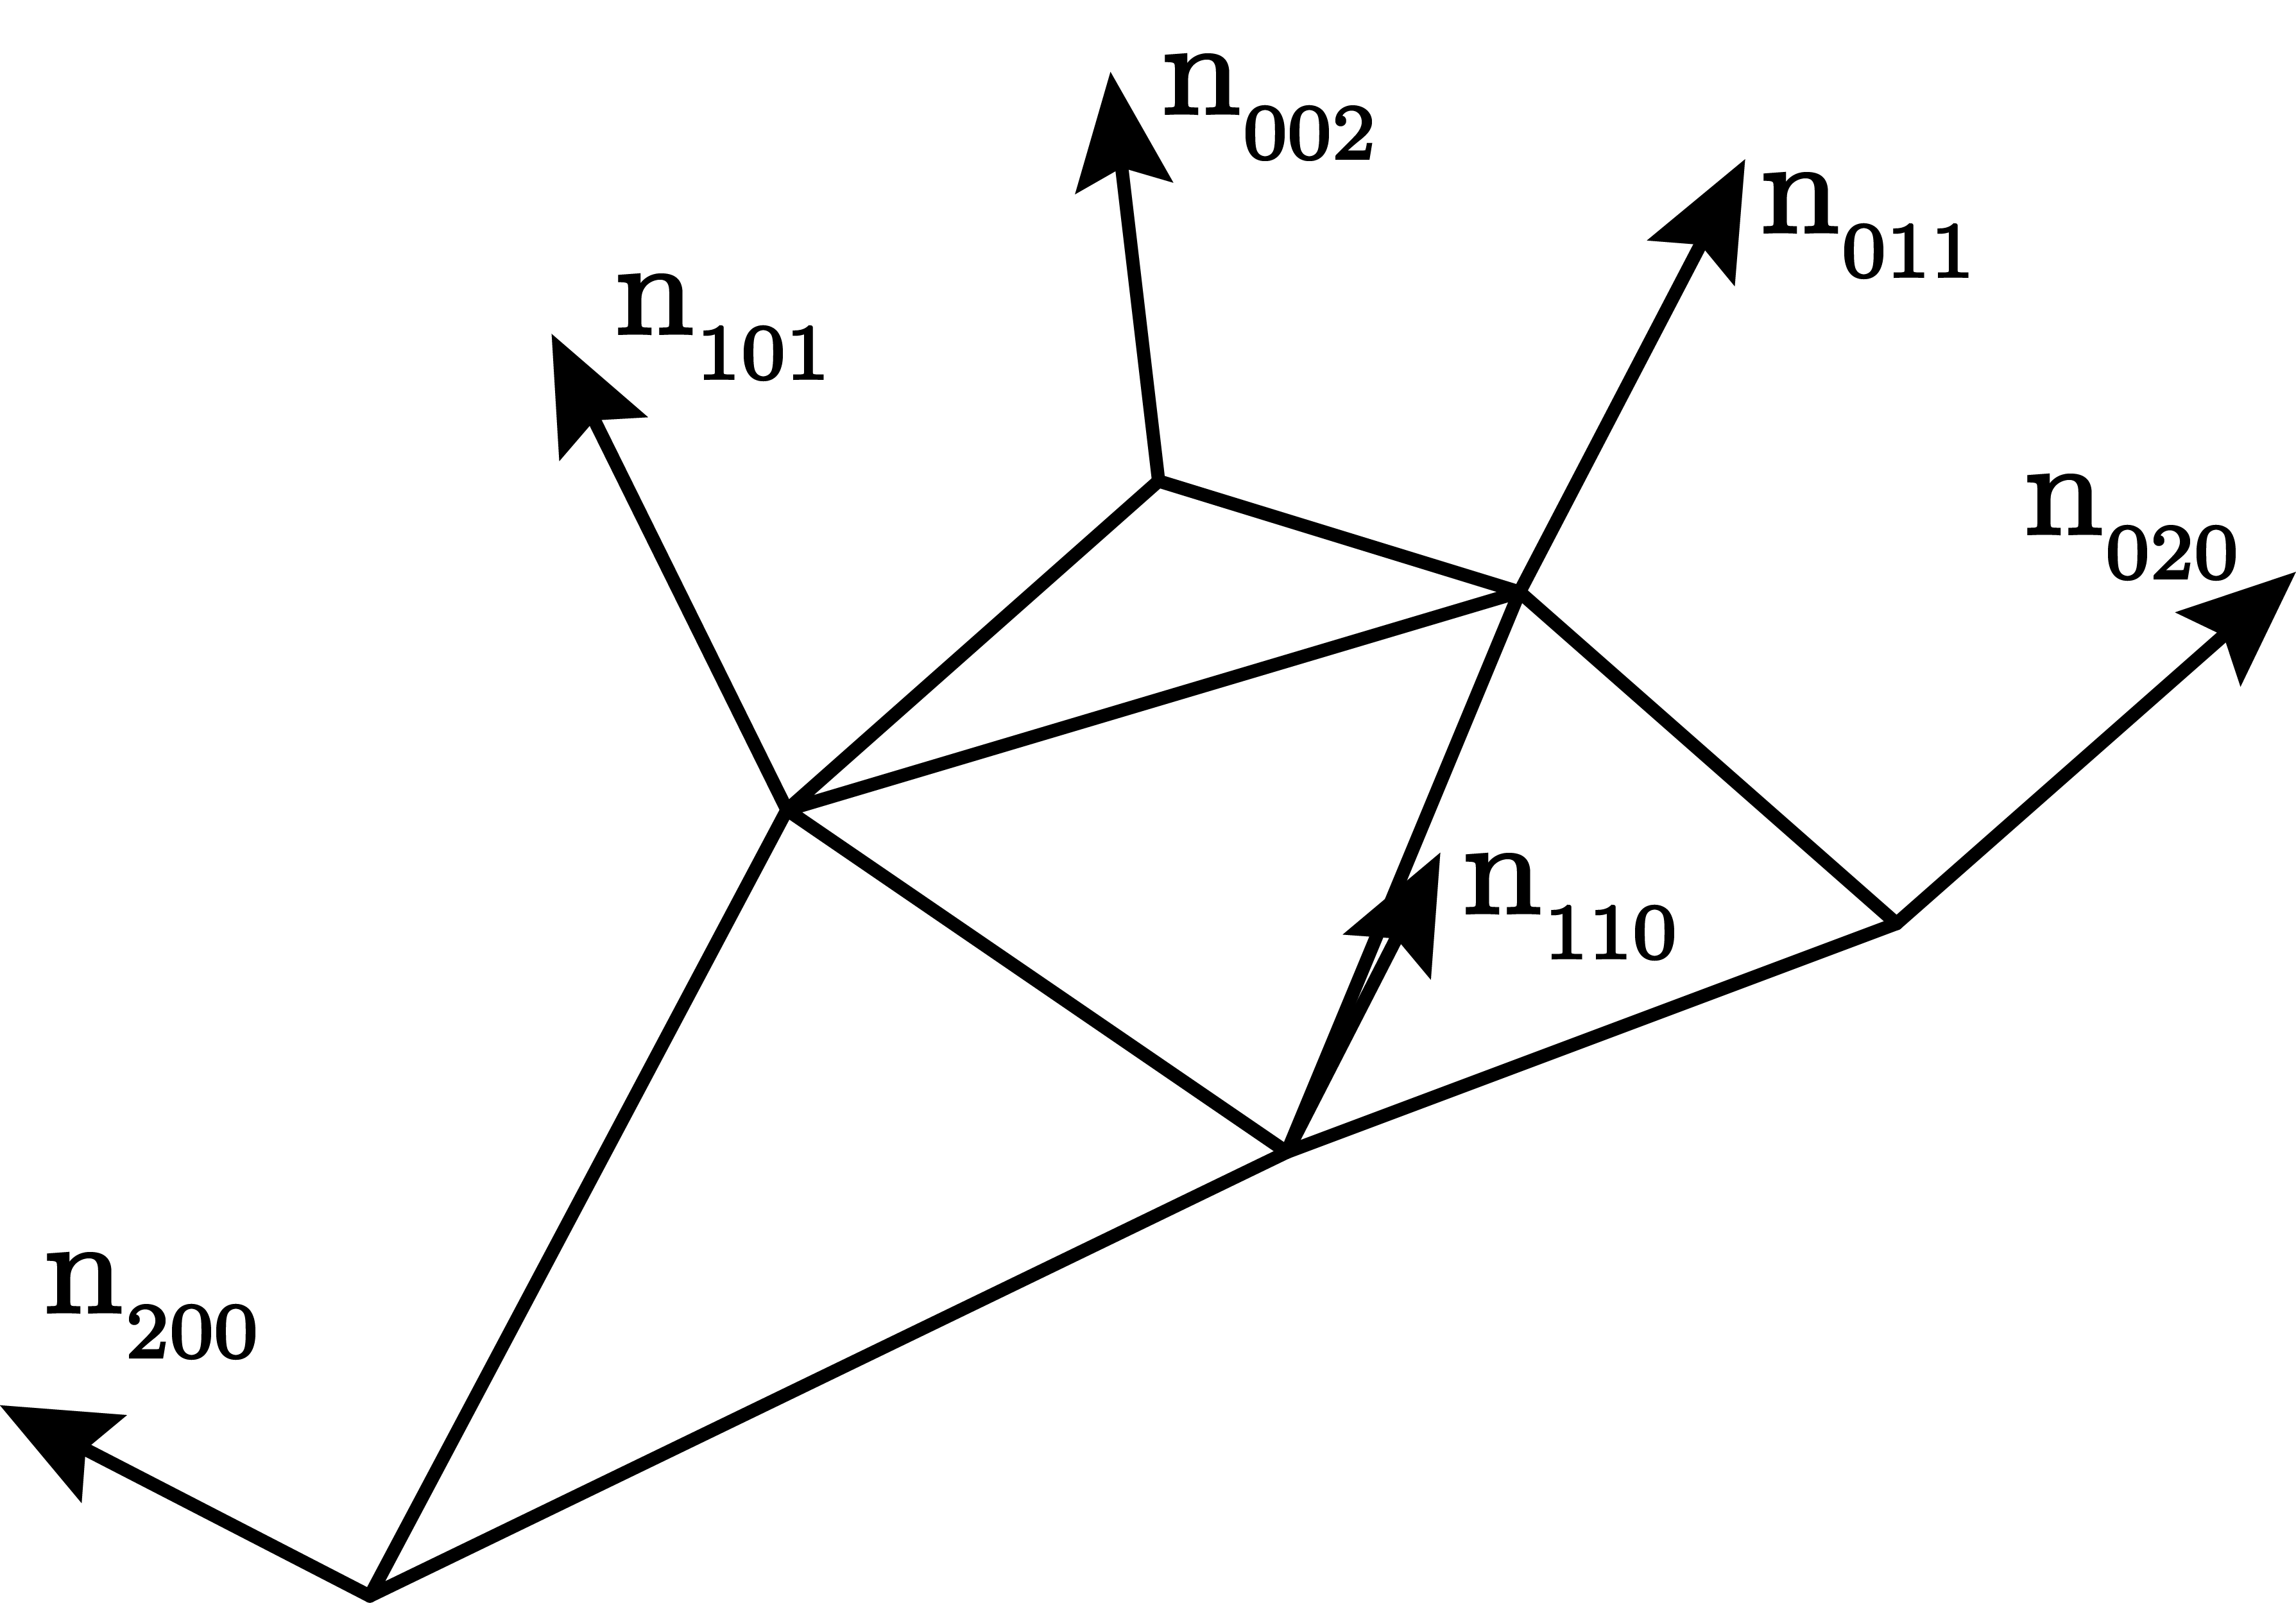
\includegraphics[width=0.45\textwidth]{./content/img/method/normals.png}
		\caption{The normal field of the point-normal triangle.}
		\label{fig:method:normal_field}
	\end{figure}

\subsubsection{Fake normals}
\label{sss:method:normals:fakeNormals}
	\citeauthor{vlachos2001curved} define the `fake' normals using a quadratic function $n(u,v)$:
	\begin{align}
		\noalign{$n(u,v): \quad R^2 \mapsto R^3,\quad$ for $w = 1 - u - v, \quad u, v, w \geq 0$}
		\begin{split}\label{eq:method:quadratic_normal_patch}
		    n(u,v) ={}& \sum_{i + j + k = 2} n_{ijk}u^i v^j w^k,\\
		      	   ={}& n_{200}w^2 + n_{020}u^2 + n_{002}v^2\\
		      	    {}& + n_{110}wu + n_{011}uv + n_{101}wv.\\
		\end{split}
	\end{align}
	The coefficients of this quadratic `patch' are the normals shown in \cref{fig:method:normal_field}. These vectors are computed for a point, halfway on every edge, i.e., $(u,v,w) = (\frac{1}{2}, \frac{1}{2}, 0)$, $(0, \frac{1}{2}, \frac{1}{2})$, $(\frac{1}{2}, 0, \frac{1}{2})$. 

	Using the function $n(u,v)$ defined in \eqref{eq:method:quadratic_normal_patch}, the normal of any point, parametrized by the barycentric coordinates $(u,v)$, can be calculated given the control net. We distinguish two types of coefficients:
	\begin{align*}
		\text{vertex coefficients: } {}&  n_{200},\ n_{020},\ n_{002} \\
		\text{edge coefficients: } {}&  n_{110},\ n_{011},\ n_{101}\\
	\end{align*}
	A vertex coefficient is simply the normal provided by the input primitive.

	An edge coefficient is calculated by taking the average of the two input vertex normals of the vertices of the edge. This results the normals presented in \cref{fig:method:normal:linear}. To capture the inflection point the average normal is then reflected across the plane perpendicular to the edge, as illustrated in \cref{fig:method:normal:reflection}. When a inflection point exists this will give the correct mid-edge normal, as shown in \cref{fig:method:normal:quadratic}. When no inflection point exists the normal field is not altered, this is illustrated in \cref{fig:method:normal:both}, where once can see that the reflection of the mid-edge normal of the curve is the mid-edge normal.

	\begin{figure}
		\centering
		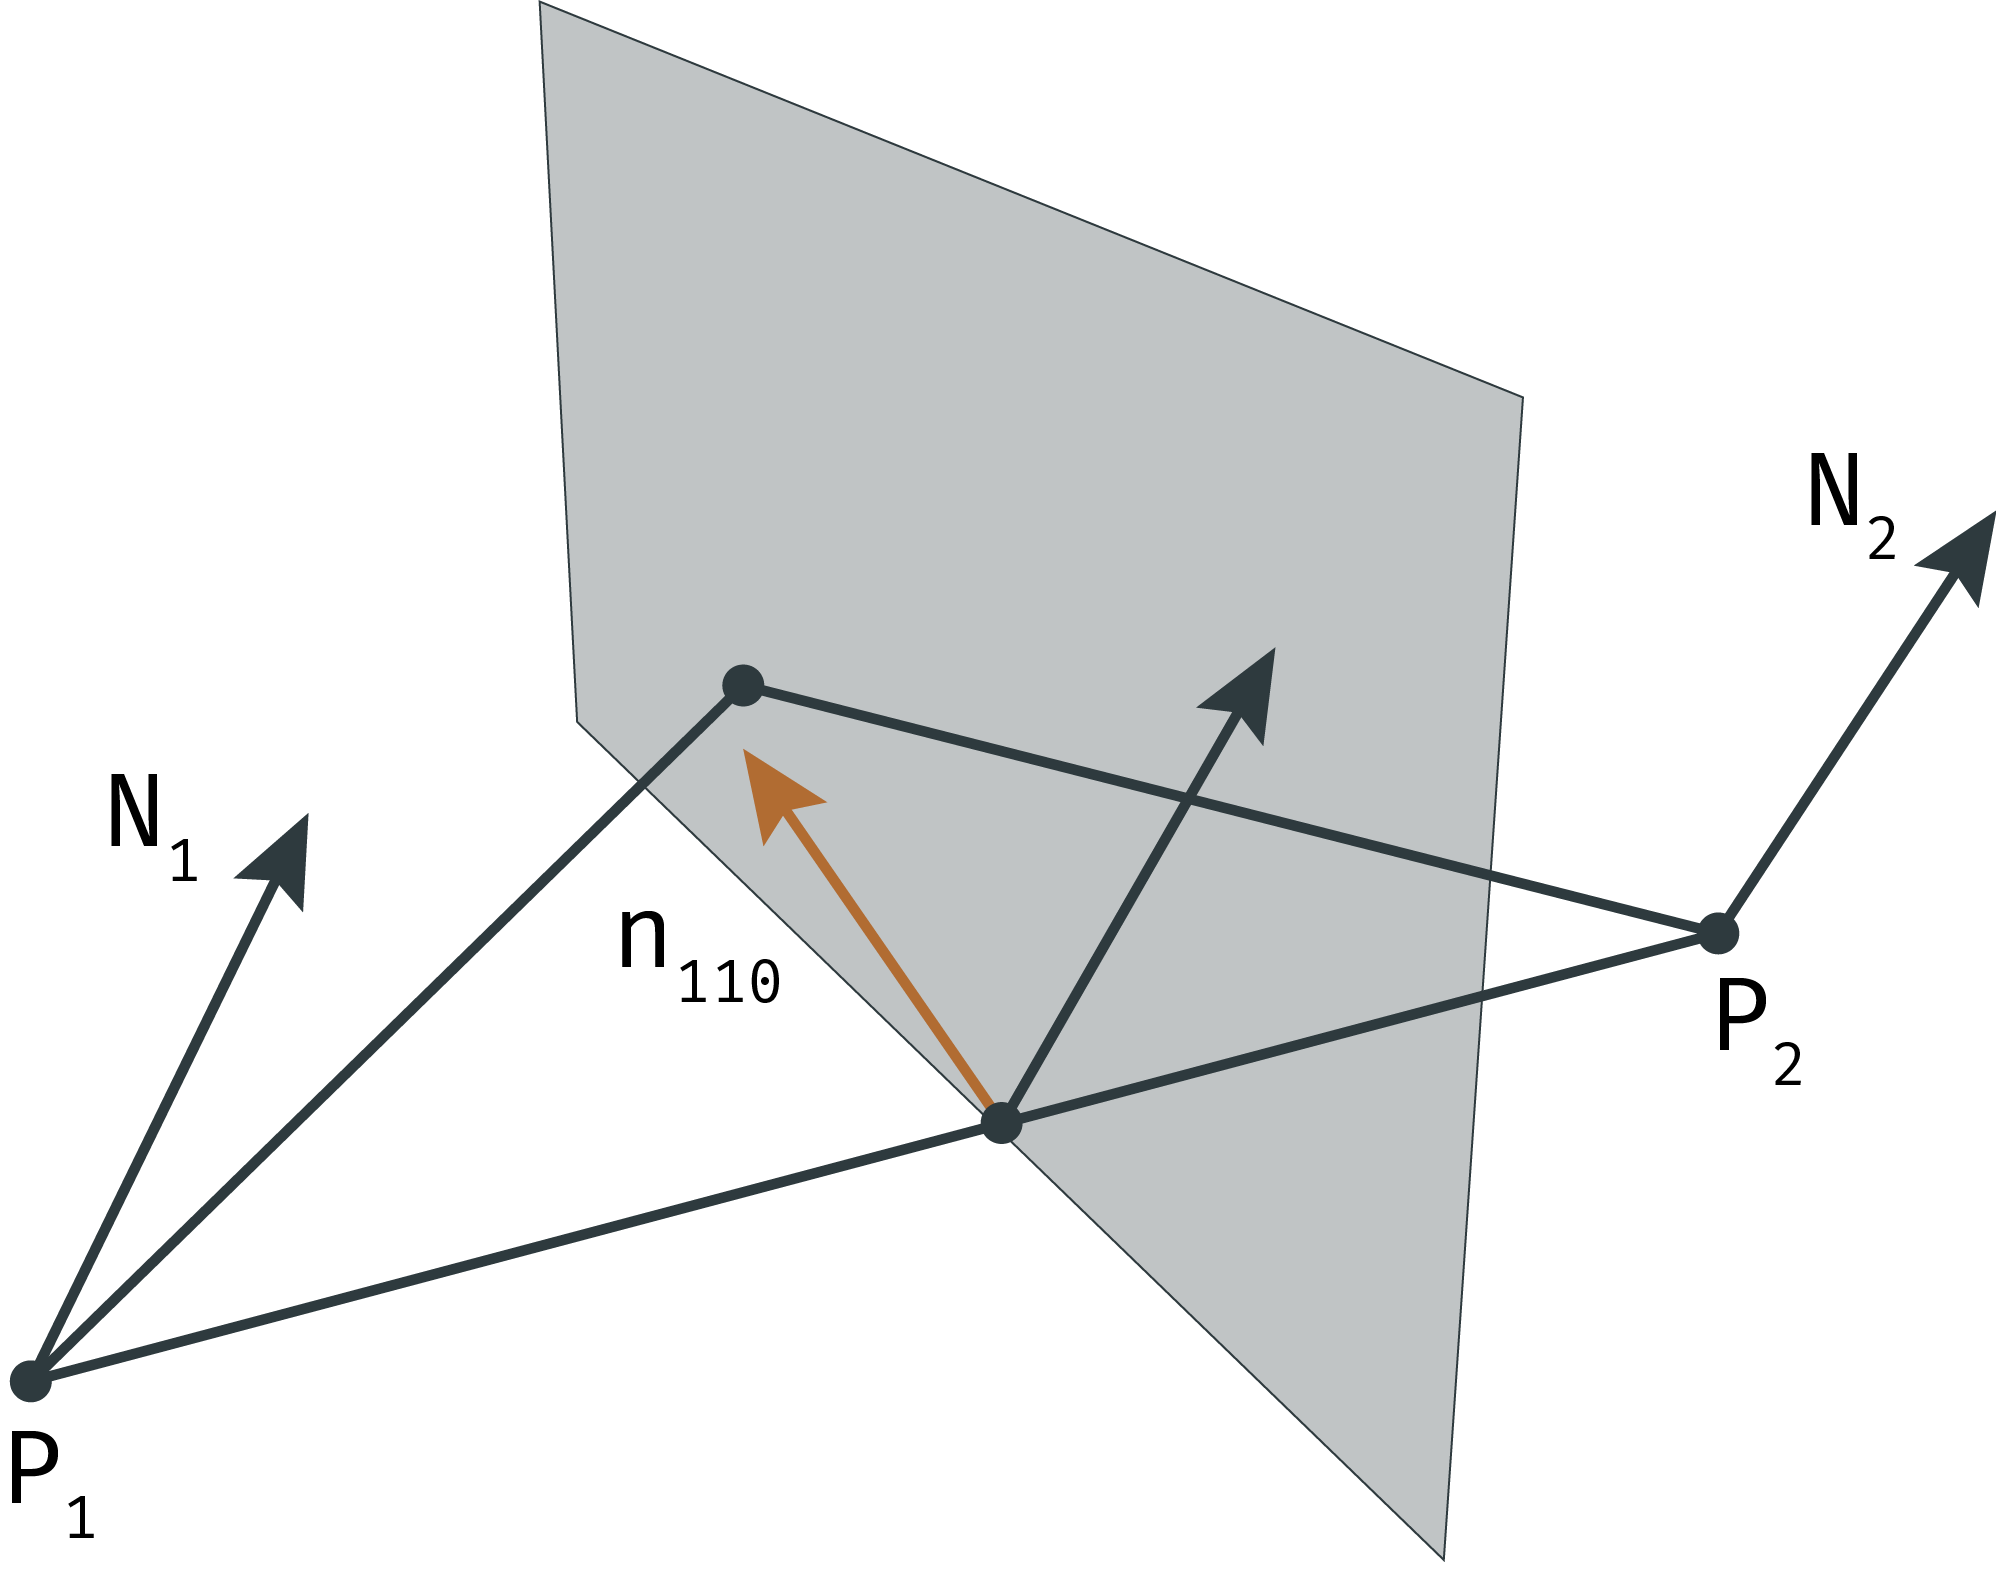
\includegraphics[width=0.45\textwidth]{./content/img/method/normal_reflection.png}
		\caption{Construction of the mid-edge normal coefficient, used for quadratically varying normals. The two input normals are averaged, which results in $n_{110}'$ and then reflected across the plane perpendicular to the edge. The resulting edge coefficient, $n_{100}$, is represented by the dashed vector. Illustration adapted from \textcite{vlachos2001curved}.}
		\label{fig:method:normal:reflection}
	\end{figure}


	% Why quadratically varying normals
	The quadratically varying normals ensure that the normal component of the PN triangles captures the inflection points, that are possible due to the cubic geometric component. 

	\Cref{fig:method:linear_vs_quadratically_varying} illustrates why one needs quadratic patches to capture these inflection points. \Cref{fig:method:normal:both} shows that when the normals point in a different direction the curve is parabolic, and no inflection point exists. In this case both linear and quadratically varying normals are able to capture the surface. \Cref{fig:method:normal:linear,fig:method:normal:quadratic} show the normals of a curve with an inflection point, approximated with linear and quadratic interpolation respectively. Observe that the linear varying normals in \cref{fig:method:normal:linear} do not capture the inflection point, i.e., the approximated normals are not sensible when one considers the curve. The quadratically varying normals in \cref{fig:method:normal:quadratic} give sensible normals, i.e, they capture the inflection point.

	\begin{figure}
		\centering
		\begin{subfigure}{\columnwidth}
			\centering
			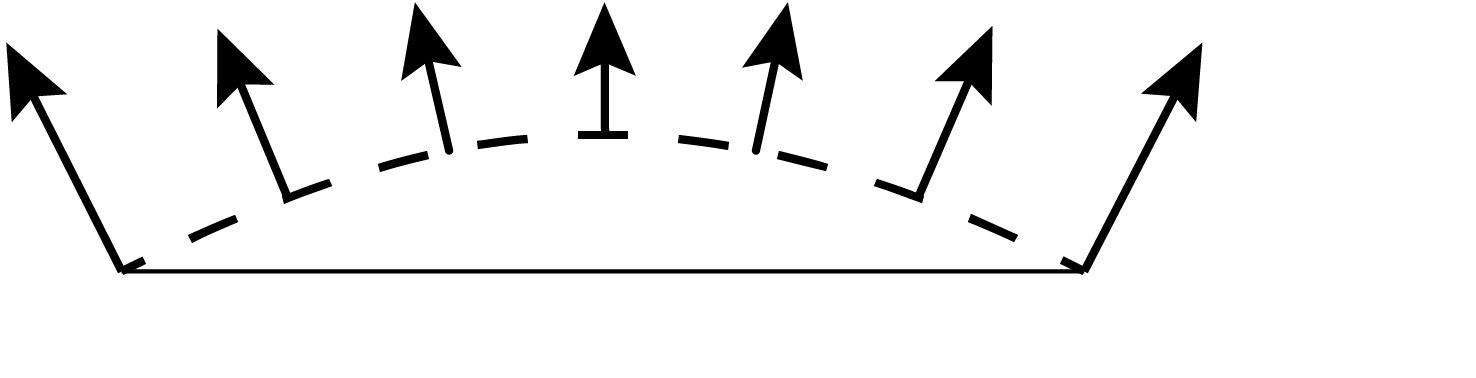
\includegraphics[width=0.8\textwidth]{./content/img/method/linearVsQuadraticNormals_both.png}
			\caption{Vector averaging with either linear or quadratic interpolation over a curve without inflections.}
			\label{fig:method:normal:both}
		\end{subfigure}
		\begin{subfigure}{\columnwidth}
			\centering
			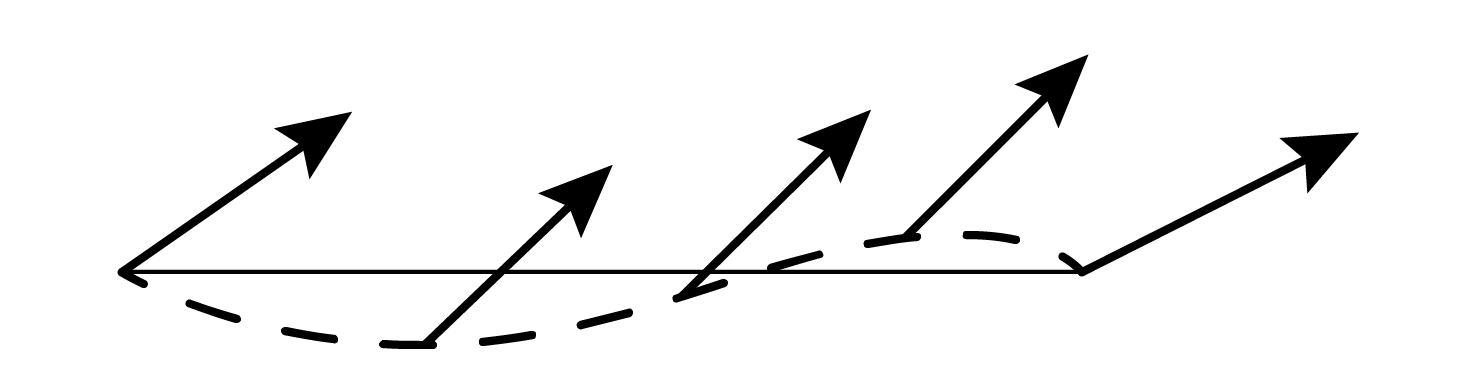
\includegraphics[width=0.8\textwidth]{./content/img/method/linearVsQuadraticNormals_linear}
			\caption{Vector averaging with linear interpolation over a curve with an inflection.}
			\label{fig:method:normal:linear}
		\end{subfigure}	
		\begin{subfigure}{\columnwidth}
			\centering
			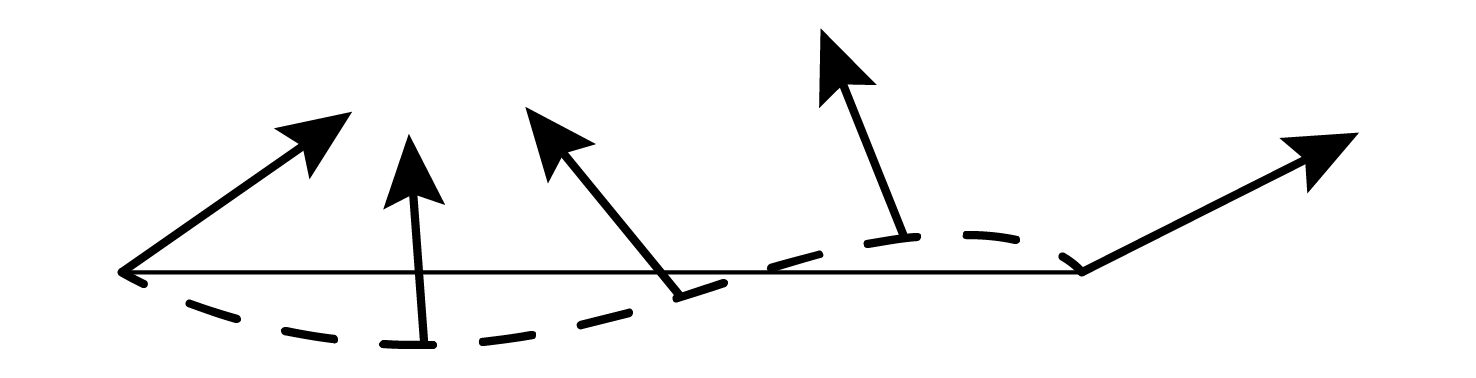
\includegraphics[width=0.8\textwidth]{./content/img/method/linearVsQuadraticNormals_quadratic}
			\caption{Vector averaging with quadratic interpolation over a curve with an inflection.}
			\label{fig:method:normal:quadratic}
		\end{subfigure}			
		\caption{Examples of normal vector averaging over an edge. The dashed lines indicate the profile of the surface that should be approximated. \subref{fig:method:normal:both} The normals of curves without inflections are correctly approximated by both linear and quadratic interpolation. The normals of a curve with inflections are incorrectly approximated with \subref{fig:method:normal:linear} linear interpolation and correctly with \subref{fig:method:normal:quadratic} interpolation. 
		\Cref{fig:method:normal:both} was adapted from \textcite{van1997phong}, \cref{fig:method:normal:linear,fig:method:normal:quadratic} from \textcite{vlachos2001curved}.}
		\label{fig:method:linear_vs_quadratically_varying}
	\end{figure}	

\subsubsection{Real normals}
\label{sss:method:normals:realNormals}
	The real normals are computed based on the geometric component of the point-normal triangle. This is done by taking the cross product of the the partial derivatives with respect to $u$ and $v$. The partial derivative of $b(u,v)$ with respect to $u$ and $v$ are respectively \cite{farin2014curves}:
	\begin{align} \label{eq:method:normal:partialU}
		\frac{\partial b(u,v)}{\partial u} ={}& \sum_{i + j + k = 2} b_{i+1, j, k} \frac{2!}{i!j!k!} u^i v^j w^k  \nonumber\\
									   ={}& w^2 b_{102} + v^2 b_{120} + u^2 b_{300} + \\
									    {}& 2 v w b_{111} + 2 u w b_{201} + 2 u v b_{210}, \nonumber
	\end{align}
	\begin{align} \label{eq:method:normal:partialV}
		\frac{\partial b(u,v)}{\partial v} ={}& \sum_{i + j + k = 2} b_{i, j + 1, k} \frac{2!}{i!j!k!}u^i v^j w^k \nonumber \\
										   ={}& w^2 b_{012} + v^2 b_{030} + u^2 b_{210} + \\
										    {}& 2 v w b_{021} + 2 u w b_{111} + 2 u v b_{120}. \nonumber
	\end{align}
	The partial derivatives define two tangent vectors in the $u$ and $v$ directions, at some point $(u,v)$ on the surface. The crossproduct of these two vectors gives us the normal of that point, as defined by the geometric component of the PN triangle.